\documentclass[1p]{elsarticle_modified}
%\bibliographystyle{elsarticle-num}

%\usepackage[colorlinks]{hyperref}
%\usepackage{abbrmath_seonhwa} %\Abb, \Ascr, \Acal ,\Abf, \Afrak
\usepackage{amsfonts}
\usepackage{amssymb}
\usepackage{amsmath}
\usepackage{amsthm}
\usepackage{scalefnt}
\usepackage{amsbsy}
\usepackage{kotex}
\usepackage{caption}
\usepackage{subfig}
\usepackage{color}
\usepackage{graphicx}
\usepackage{xcolor} %% white, black, red, green, blue, cyan, magenta, yellow
\usepackage{float}
\usepackage{setspace}
\usepackage{hyperref}

\usepackage{tikz}
\usetikzlibrary{arrows}

\usepackage{multirow}
\usepackage{array} % fixed length table
\usepackage{hhline}

%%%%%%%%%%%%%%%%%%%%%
\makeatletter
\renewcommand*\env@matrix[1][\arraystretch]{%
	\edef\arraystretch{#1}%
	\hskip -\arraycolsep
	\let\@ifnextchar\new@ifnextchar
	\array{*\c@MaxMatrixCols c}}
\makeatother %https://tex.stackexchange.com/questions/14071/how-can-i-increase-the-line-spacing-in-a-matrix
%%%%%%%%%%%%%%%

\usepackage[normalem]{ulem}

\newcommand{\msout}[1]{\ifmmode\text{\sout{\ensuremath{#1}}}\else\sout{#1}\fi}
%SOURCE: \msout is \stkout macro in https://tex.stackexchange.com/questions/20609/strikeout-in-math-mode

\newcommand{\cancel}[1]{
	\ifmmode
	{\color{red}\msout{#1}}
	\else
	{\color{red}\sout{#1}}
	\fi
}

\newcommand{\add}[1]{
	{\color{blue}\uwave{#1}}
}

\newcommand{\replace}[2]{
	\ifmmode
	{\color{red}\msout{#1}}{\color{blue}\uwave{#2}}
	\else
	{\color{red}\sout{#1}}{\color{blue}\uwave{#2}}
	\fi
}

\newcommand{\Sol}{\mathcal{S}} %segment
\newcommand{\D}{D} %diagram
\newcommand{\A}{\mathcal{A}} %arc


%%%%%%%%%%%%%%%%%%%%%%%%%%%%%5 test

\def\sl{\operatorname{\textup{SL}}(2,\Cbb)}
\def\psl{\operatorname{\textup{PSL}}(2,\Cbb)}
\def\quan{\mkern 1mu \triangleright \mkern 1mu}

\theoremstyle{definition}
\newtheorem{thm}{Theorem}[section]
\newtheorem{prop}[thm]{Proposition}
\newtheorem{lem}[thm]{Lemma}
\newtheorem{ques}[thm]{Question}
\newtheorem{cor}[thm]{Corollary}
\newtheorem{defn}[thm]{Definition}
\newtheorem{exam}[thm]{Example}
\newtheorem{rmk}[thm]{Remark}
\newtheorem{alg}[thm]{Algorithm}

\newcommand{\I}{\sqrt{-1}}
\begin{document}

%\begin{frontmatter}
%
%\title{Boundary parabolic representations of knots up to 8 crossings}
%
%%% Group authors per affiliation:
%\author{Yunhi Cho} 
%\address{Department of Mathematics, University of Seoul, Seoul, Korea}
%\ead{yhcho@uos.ac.kr}
%
%
%\author{Seonhwa Kim} %\fnref{s_kim}}
%\address{Center for Geometry and Physics, Institute for Basic Science, Pohang, 37673, Korea}
%\ead{ryeona17@ibs.re.kr}
%
%\author{Hyuk Kim}
%\address{Department of Mathematical Sciences, Seoul National University, Seoul 08826, Korea}
%\ead{hyukkim@snu.ac.kr}
%
%\author{Seokbeom Yoon}
%\address{Department of Mathematical Sciences, Seoul National University, Seoul, 08826,  Korea}
%\ead{sbyoon15@snu.ac.kr}
%
%\begin{abstract}
%We find all boundary parabolic representation of knots up to 8 crossings.
%
%\end{abstract}
%\begin{keyword}
%    \MSC[2010] 57M25 
%\end{keyword}
%
%\end{frontmatter}

%\linenumbers
%\tableofcontents
%
\newcommand\colored[1]{\textcolor{white}{\rule[-0.35ex]{0.8em}{1.4ex}}\kern-0.8em\color{red} #1}%
%\newcommand\colored[1]{\textcolor{white}{ #1}\kern-2.17ex	\textcolor{white}{ #1}\kern-1.81ex	\textcolor{white}{ #1}\kern-2.15ex\color{red}#1	}

{\Large $\underline{12a_{1064}~(K12a_{1064})}$}

\setlength{\tabcolsep}{10pt}
\renewcommand{\arraystretch}{1.6}
\vspace{1cm}\begin{tabular}{m{100pt}>{\centering\arraybackslash}m{274pt}}
\multirow{5}{120pt}{
	\centering
	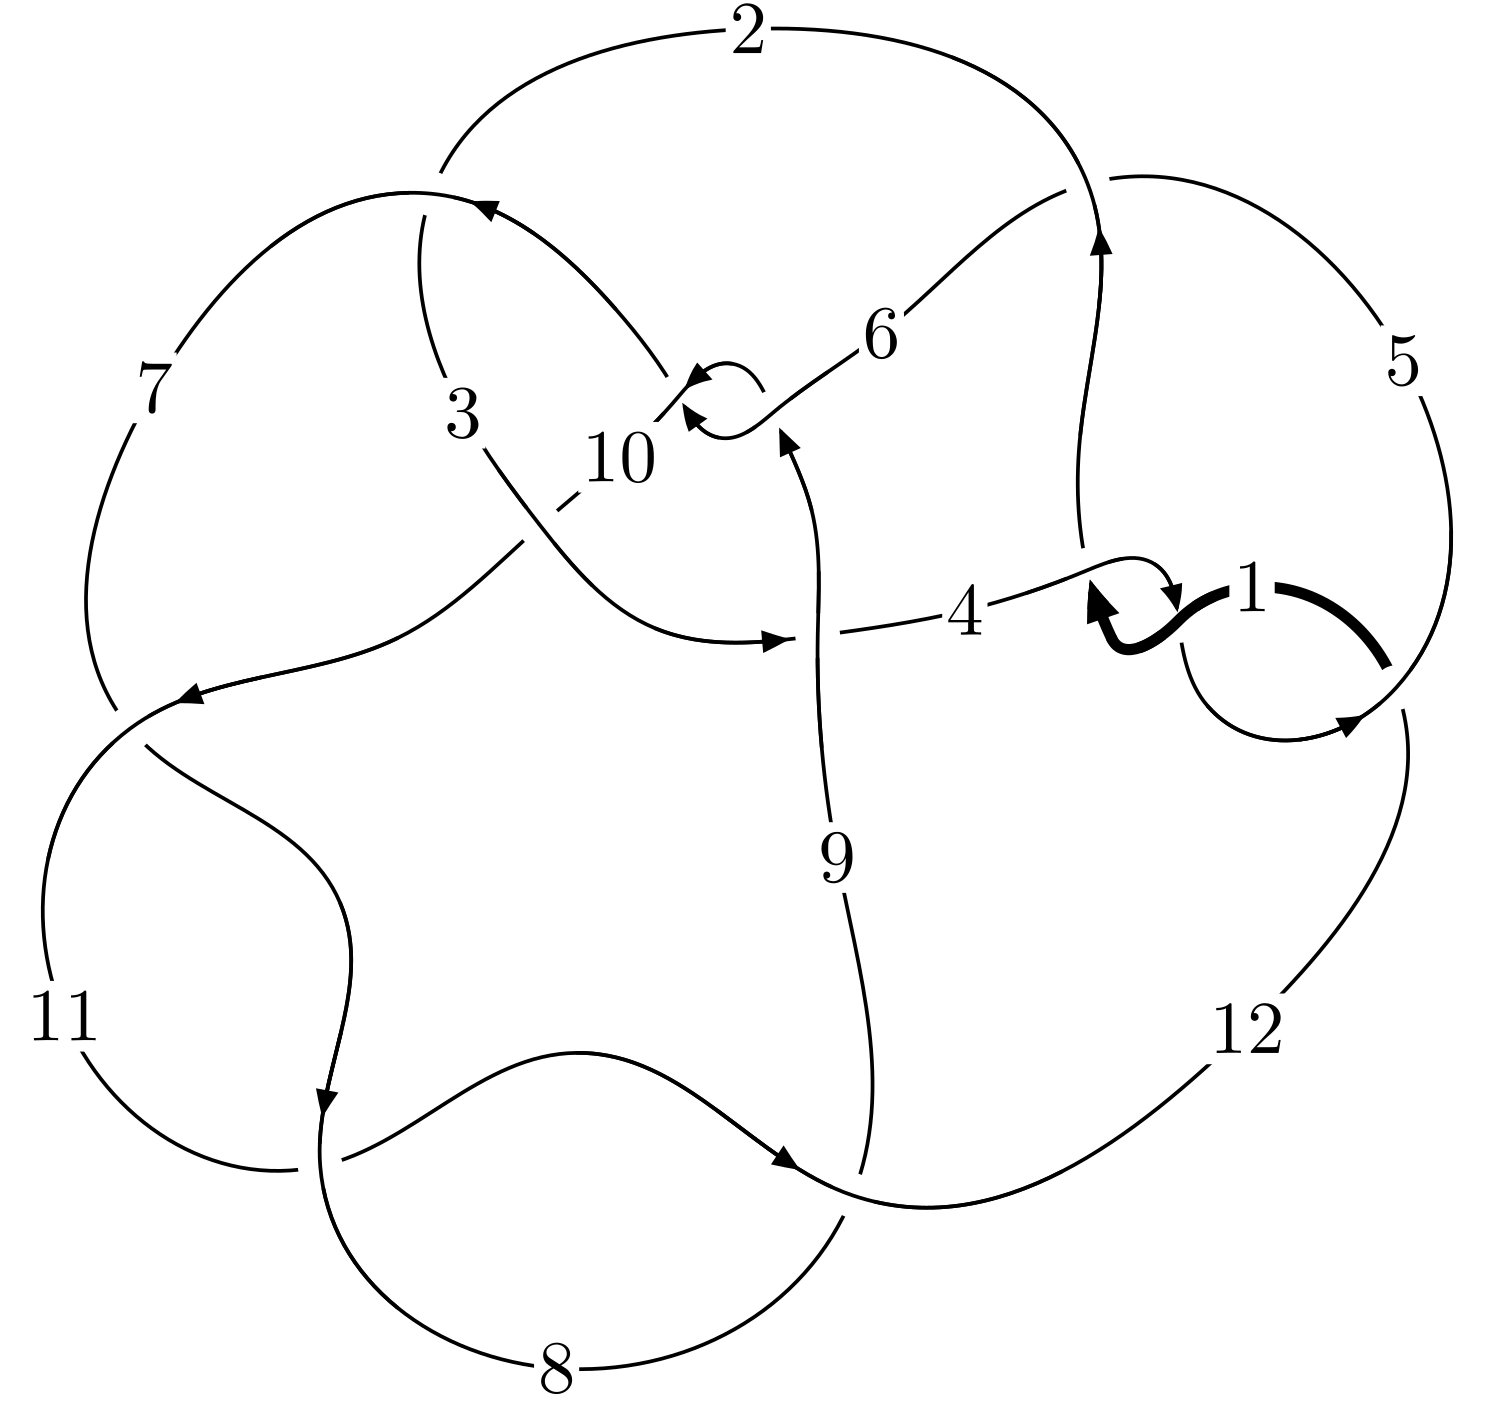
\includegraphics[width=112pt]{../../../GIT/diagram.site/Diagrams/png/1865_12a_1064.png}\\
\ \ \ A knot diagram\footnotemark}&
\allowdisplaybreaks
\textbf{Linearized knot diagam} \\
\cline{2-2}
 &
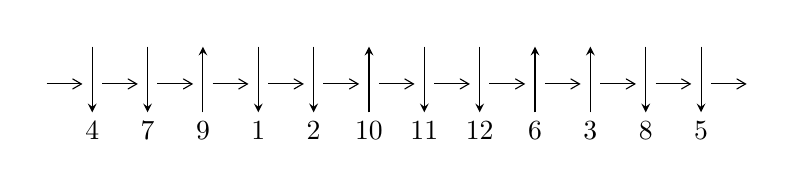
\begin{tikzpicture}[x=20pt, y=17pt]
	% nodes
	\node (C0) at (0, 0) {};
	\node (C1) at (1, 0) {};
	\node (C1U) at (1, +1) {};
	\node (C1D) at (1, -1) {4};

	\node (C2) at (2, 0) {};
	\node (C2U) at (2, +1) {};
	\node (C2D) at (2, -1) {7};

	\node (C3) at (3, 0) {};
	\node (C3U) at (3, +1) {};
	\node (C3D) at (3, -1) {9};

	\node (C4) at (4, 0) {};
	\node (C4U) at (4, +1) {};
	\node (C4D) at (4, -1) {1};

	\node (C5) at (5, 0) {};
	\node (C5U) at (5, +1) {};
	\node (C5D) at (5, -1) {2};

	\node (C6) at (6, 0) {};
	\node (C6U) at (6, +1) {};
	\node (C6D) at (6, -1) {10};

	\node (C7) at (7, 0) {};
	\node (C7U) at (7, +1) {};
	\node (C7D) at (7, -1) {11};

	\node (C8) at (8, 0) {};
	\node (C8U) at (8, +1) {};
	\node (C8D) at (8, -1) {12};

	\node (C9) at (9, 0) {};
	\node (C9U) at (9, +1) {};
	\node (C9D) at (9, -1) {6};

	\node (C10) at (10, 0) {};
	\node (C10U) at (10, +1) {};
	\node (C10D) at (10, -1) {3};

	\node (C11) at (11, 0) {};
	\node (C11U) at (11, +1) {};
	\node (C11D) at (11, -1) {8};

	\node (C12) at (12, 0) {};
	\node (C12U) at (12, +1) {};
	\node (C12D) at (12, -1) {5};
	\node (C13) at (13, 0) {};

	% arrows
	\draw[->,>={angle 60}]
	(C0) edge (C1) (C1) edge (C2) (C2) edge (C3) (C3) edge (C4) (C4) edge (C5) (C5) edge (C6) (C6) edge (C7) (C7) edge (C8) (C8) edge (C9) (C9) edge (C10) (C10) edge (C11) (C11) edge (C12) (C12) edge (C13) ;	\draw[->,>=stealth]
	(C1U) edge (C1D) (C2U) edge (C2D) (C3D) edge (C3U) (C4U) edge (C4D) (C5U) edge (C5D) (C6D) edge (C6U) (C7U) edge (C7D) (C8U) edge (C8D) (C9D) edge (C9U) (C10D) edge (C10U) (C11U) edge (C11D) (C12U) edge (C12D) ;
	\end{tikzpicture} \\
\hhline{~~} \\& 
\textbf{Solving Sequence} \\ \cline{2-2} 
 &
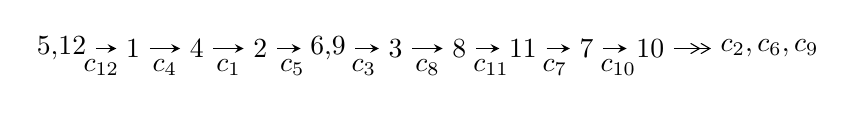
\begin{tikzpicture}[x=23pt, y=7pt]
	% node
	\node (A0) at (-1/8, 0) {5,12};
	\node (A1) at (1, 0) {1};
	\node (A2) at (2, 0) {4};
	\node (A3) at (3, 0) {2};
	\node (A4) at (65/16, 0) {6,9};
	\node (A5) at (41/8, 0) {3};
	\node (A6) at (49/8, 0) {8};
	\node (A7) at (57/8, 0) {11};
	\node (A8) at (65/8, 0) {7};
	\node (A9) at (73/8, 0) {10};
	\node (C1) at (1/2, -1) {$c_{12}$};
	\node (C2) at (3/2, -1) {$c_{4}$};
	\node (C3) at (5/2, -1) {$c_{1}$};
	\node (C4) at (7/2, -1) {$c_{5}$};
	\node (C5) at (37/8, -1) {$c_{3}$};
	\node (C6) at (45/8, -1) {$c_{8}$};
	\node (C7) at (53/8, -1) {$c_{11}$};
	\node (C8) at (61/8, -1) {$c_{7}$};
	\node (C9) at (69/8, -1) {$c_{10}$};
	\node (A10) at (11, 0) {$c_{2},c_{6},c_{9}$};

	% edge
	\draw[->,>=stealth]	
	(A0) edge (A1) (A1) edge (A2) (A2) edge (A3) (A3) edge (A4) (A4) edge (A5) (A5) edge (A6) (A6) edge (A7) (A7) edge (A8) (A8) edge (A9) ;
	\draw[->>,>={angle 60}]	
	(A9) edge (A10);
\end{tikzpicture} \\ 

\end{tabular} \\

\footnotetext{
The image of knot diagram is generated by the software ``\textbf{Draw programme}" developed by Andrew Bartholomew(\url{http://www.layer8.co.uk/maths/draw/index.htm\#Running-draw}), where we modified some parts for our purpose(\url{https://github.com/CATsTAILs/LinksPainter}).
}\phantom \\ \newline 
\centering \textbf{Ideals for irreducible components\footnotemark of $X_{\text{par}}$} 
 
\begin{align*}
I^u_{1}&=\langle 
-2.52109\times10^{85} u^{82}+8.64634\times10^{85} u^{81}+\cdots+1.02529\times10^{87} b+1.52237\times10^{87},\\
\phantom{I^u_{1}}&\phantom{= \langle  }-1.47090\times10^{87} u^{82}-1.63708\times10^{87} u^{81}+\cdots+1.02529\times10^{87} a-7.79066\times10^{86},\;u^{83}+u^{82}+\cdots-2 u-1\rangle \\
\\
\end{align*}
\raggedright * 1 irreducible components of $\dim_{\mathbb{C}}=0$, with total 83 representations.\\
\footnotetext{All coefficients of polynomials are rational numbers. But the coefficients are sometimes approximated in decimal forms when there is not enough margin.}
\newpage
\renewcommand{\arraystretch}{1}
\centering \section*{I. $I^u_{1}= \langle -2.52\times10^{85} u^{82}+8.65\times10^{85} u^{81}+\cdots+1.03\times10^{87} b+1.52\times10^{87},\;-1.47\times10^{87} u^{82}-1.64\times10^{87} u^{81}+\cdots+1.03\times10^{87} a-7.79\times10^{86},\;u^{83}+u^{82}+\cdots-2 u-1 \rangle$}
\flushleft \textbf{(i) Arc colorings}\\
\begin{tabular}{m{7pt} m{180pt} m{7pt} m{180pt} }
\flushright $a_{5}=$&$\begin{pmatrix}0\\u\end{pmatrix}$ \\
\flushright $a_{12}=$&$\begin{pmatrix}1\\0\end{pmatrix}$ \\
\flushright $a_{1}=$&$\begin{pmatrix}1\\u^2\end{pmatrix}$ \\
\flushright $a_{4}=$&$\begin{pmatrix}u\\u^3+u\end{pmatrix}$ \\
\flushright $a_{2}=$&$\begin{pmatrix}u^2+1\\u^4+2 u^2\end{pmatrix}$ \\
\flushright $a_{6}=$&$\begin{pmatrix}- u^5-2 u^3- u\\- u^7-3 u^5-2 u^3+u\end{pmatrix}$ \\
\flushright $a_{9}=$&$\begin{pmatrix}1.43461 u^{82}+1.59669 u^{81}+\cdots-48.1974 u+0.759849\\0.0245891 u^{82}-0.0843305 u^{81}+\cdots-0.539171 u-1.48482\end{pmatrix}$ \\
\flushright $a_{3}=$&$\begin{pmatrix}-3.85435 u^{82}-3.70576 u^{81}+\cdots+12.1010 u-10.3867\\-0.109874 u^{82}-0.158192 u^{81}+\cdots+6.49193 u+1.37180\end{pmatrix}$ \\
\flushright $a_{8}=$&$\begin{pmatrix}1.45920 u^{82}+1.51236 u^{81}+\cdots-48.7366 u-0.724973\\0.0245891 u^{82}-0.0843305 u^{81}+\cdots-0.539171 u-1.48482\end{pmatrix}$ \\
\flushright $a_{11}=$&$\begin{pmatrix}1.57618 u^{82}+0.907236 u^{81}+\cdots-69.1885 u-0.00842359\\-0.0277634 u^{82}-0.0657480 u^{81}+\cdots-1.84911 u-2.19386\end{pmatrix}$ \\
\flushright $a_{7}=$&$\begin{pmatrix}-1.40639 u^{82}-1.36785 u^{81}+\cdots+42.0418 u-2.35067\\0.0598792 u^{82}-0.104829 u^{81}+\cdots+2.65151 u+1.36301\end{pmatrix}$ \\
\flushright $a_{10}=$&$\begin{pmatrix}1.48382 u^{82}+1.56199 u^{81}+\cdots-47.0880 u+0.730578\\0.0160101 u^{82}-0.00198206 u^{81}+\cdots-1.69531 u-1.51353\end{pmatrix}$\\&\end{tabular}
\flushleft \textbf{(ii) Obstruction class $= -1$}\\~\\
\flushleft \textbf{(iii) Cusp Shapes $= 3.75821 u^{82}+4.13643 u^{81}+\cdots-2.88911 u-1.93224$}\\~\\
\newpage\renewcommand{\arraystretch}{1}
\flushleft \textbf{(iv) u-Polynomials at the component}\newline \\
\begin{tabular}{m{50pt}|m{274pt}}
Crossings & \hspace{64pt}u-Polynomials at each crossing \\
\hline $$\begin{aligned}c_{1},c_{4},c_{12}\end{aligned}$$&$\begin{aligned}
&u^{83}- u^{82}+\cdots-2 u+1
\end{aligned}$\\
\hline $$\begin{aligned}c_{2}\end{aligned}$$&$\begin{aligned}
&u^{83}-3 u^{82}+\cdots-8 u-97
\end{aligned}$\\
\hline $$\begin{aligned}c_{3}\end{aligned}$$&$\begin{aligned}
&u^{83}- u^{82}+\cdots-29240 u-5563
\end{aligned}$\\
\hline $$\begin{aligned}c_{5}\end{aligned}$$&$\begin{aligned}
&u^{83}+u^{82}+\cdots+9630 u+2689
\end{aligned}$\\
\hline $$\begin{aligned}c_{6},c_{9}\end{aligned}$$&$\begin{aligned}
&u^{83}- u^{82}+\cdots-7 u^2+1
\end{aligned}$\\
\hline $$\begin{aligned}c_{7},c_{8},c_{11}\end{aligned}$$&$\begin{aligned}
&u^{83}+7 u^{82}+\cdots+7 u^2-1
\end{aligned}$\\
\hline $$\begin{aligned}c_{10}\end{aligned}$$&$\begin{aligned}
&u^{83}+3 u^{82}+\cdots-4 u-1
\end{aligned}$\\
\hline
\end{tabular}\\~\\
\newpage\renewcommand{\arraystretch}{1}
\flushleft \textbf{(v) Riley Polynomials at the component}\newline \\
\begin{tabular}{m{50pt}|m{274pt}}
Crossings & \hspace{64pt}Riley Polynomials at each crossing \\
\hline $$\begin{aligned}c_{1},c_{4},c_{12}\end{aligned}$$&$\begin{aligned}
&y^{83}+71 y^{82}+\cdots-102 y-1
\end{aligned}$\\
\hline $$\begin{aligned}c_{2}\end{aligned}$$&$\begin{aligned}
&y^{83}-513 y^{82}+\cdots+637742 y-9409
\end{aligned}$\\
\hline $$\begin{aligned}c_{3}\end{aligned}$$&$\begin{aligned}
&y^{83}-533 y^{82}+\cdots+2125110634 y-30946969
\end{aligned}$\\
\hline $$\begin{aligned}c_{5}\end{aligned}$$&$\begin{aligned}
&y^{83}-29 y^{82}+\cdots-827229158 y-7230721
\end{aligned}$\\
\hline $$\begin{aligned}c_{6},c_{9}\end{aligned}$$&$\begin{aligned}
&y^{83}-53 y^{82}+\cdots+14 y-1
\end{aligned}$\\
\hline $$\begin{aligned}c_{7},c_{8},c_{11}\end{aligned}$$&$\begin{aligned}
&y^{83}-85 y^{82}+\cdots+14 y-1
\end{aligned}$\\
\hline $$\begin{aligned}c_{10}\end{aligned}$$&$\begin{aligned}
&y^{83}+7 y^{82}+\cdots+66 y-1
\end{aligned}$\\
\hline
\end{tabular}\\~\\
\newpage\flushleft \textbf{(vi) Complex Volumes and Cusp Shapes}
$$\begin{array}{c|c|c}  
\text{Solutions to }I^u_{1}& \I (\text{vol} + \sqrt{-1}CS) & \text{Cusp shape}\\
 \hline 
\begin{aligned}
u &= \phantom{-}0.904665 + 0.431308 I \\
a &= \phantom{-}0.444111 - 0.833130 I \\
b &= \phantom{-}1.48483 + 0.03450 I\end{aligned}
 & -6.93263 - 2.69856 I & \phantom{-0.000000 } 0 \\ \hline\begin{aligned}
u &= \phantom{-}0.904665 - 0.431308 I \\
a &= \phantom{-}0.444111 + 0.833130 I \\
b &= \phantom{-}1.48483 - 0.03450 I\end{aligned}
 & -6.93263 + 2.69856 I & \phantom{-0.000000 } 0 \\ \hline\begin{aligned}
u &= -0.523171 + 0.935123 I \\
a &= \phantom{-}0.078517 - 0.193819 I \\
b &= -1.53601 - 0.20823 I\end{aligned}
 & -4.33446 - 7.80527 I & \phantom{-0.000000 } 0 \\ \hline\begin{aligned}
u &= -0.523171 - 0.935123 I \\
a &= \phantom{-}0.078517 + 0.193819 I \\
b &= -1.53601 + 0.20823 I\end{aligned}
 & -4.33446 + 7.80527 I & \phantom{-0.000000 } 0 \\ \hline\begin{aligned}
u &= \phantom{-}0.926387 + 0.043053 I \\
a &= -1.253500 + 0.168894 I \\
b &= -1.47810 - 0.00383 I\end{aligned}
 & -7.59406 - 0.00917 I & -13.41457 + 0. I\phantom{ +0.000000I} \\ \hline\begin{aligned}
u &= \phantom{-}0.926387 - 0.043053 I \\
a &= -1.253500 - 0.168894 I \\
b &= -1.47810 + 0.00383 I\end{aligned}
 & -7.59406 + 0.00917 I & -13.41457 + 0. I\phantom{ +0.000000I} \\ \hline\begin{aligned}
u &= -0.387244 + 0.823860 I \\
a &= -0.565051 - 0.405945 I \\
b &= \phantom{-}0.547345 + 0.608594 I\end{aligned}
 & \phantom{-}2.54832 - 4.77196 I & \phantom{-0.000000 -}0. + 4.88934 I \\ \hline\begin{aligned}
u &= -0.387244 - 0.823860 I \\
a &= -0.565051 + 0.405945 I \\
b &= \phantom{-}0.547345 - 0.608594 I\end{aligned}
 & \phantom{-}2.54832 + 4.77196 I & \phantom{-0.000000 } 0. - 4.88934 I \\ \hline\begin{aligned}
u &= -0.371273 + 1.048980 I \\
a &= -0.208988 + 0.342891 I \\
b &= \phantom{-}1.56520 + 0.18830 I\end{aligned}
 & -7.61151 - 2.62136 I & \phantom{-0.000000 } 0 \\ \hline\begin{aligned}
u &= -0.371273 - 1.048980 I \\
a &= -0.208988 - 0.342891 I \\
b &= \phantom{-}1.56520 - 0.18830 I\end{aligned}
 & -7.61151 + 2.62136 I & \phantom{-0.000000 } 0\\
 \hline 
 \end{array}$$\newpage$$\begin{array}{c|c|c}  
\text{Solutions to }I^u_{1}& \I (\text{vol} + \sqrt{-1}CS) & \text{Cusp shape}\\
 \hline 
\begin{aligned}
u &= -0.849324 + 0.250360 I \\
a &= -1.03559 - 1.28238 I \\
b &= -1.55846 + 0.25137 I\end{aligned}
 & -6.4541 + 12.6262 I & -7.38891 - 7.59104 I \\ \hline\begin{aligned}
u &= -0.849324 - 0.250360 I \\
a &= -1.03559 + 1.28238 I \\
b &= -1.55846 - 0.25137 I\end{aligned}
 & -6.4541 - 12.6262 I & -7.38891 + 7.59104 I \\ \hline\begin{aligned}
u &= \phantom{-}0.349735 + 1.067780 I \\
a &= -0.248736 - 0.432337 I \\
b &= \phantom{-}0.508066 + 0.276673 I\end{aligned}
 & \phantom{-}1.92187 - 4.22604 I & \phantom{-0.000000 } 0 \\ \hline\begin{aligned}
u &= \phantom{-}0.349735 - 1.067780 I \\
a &= -0.248736 + 0.432337 I \\
b &= \phantom{-}0.508066 - 0.276673 I\end{aligned}
 & \phantom{-}1.92187 + 4.22604 I & \phantom{-0.000000 } 0 \\ \hline\begin{aligned}
u &= -0.801322 + 0.161892 I \\
a &= \phantom{-}1.19606 + 1.08916 I \\
b &= \phantom{-}1.57257 - 0.25982 I\end{aligned}
 & -10.32350 + 6.88913 I & -11.30755 - 5.10720 I \\ \hline\begin{aligned}
u &= -0.801322 - 0.161892 I \\
a &= \phantom{-}1.19606 - 1.08916 I \\
b &= \phantom{-}1.57257 + 0.25982 I\end{aligned}
 & -10.32350 - 6.88913 I & -11.30755 + 5.10720 I \\ \hline\begin{aligned}
u &= \phantom{-}0.527206 + 0.622474 I \\
a &= -0.213152 - 0.852381 I \\
b &= \phantom{-}1.47354 + 0.06068 I\end{aligned}
 & -6.26479 - 2.24210 I & -10.47377 + 2.86125 I \\ \hline\begin{aligned}
u &= \phantom{-}0.527206 - 0.622474 I \\
a &= -0.213152 + 0.852381 I \\
b &= \phantom{-}1.47354 - 0.06068 I\end{aligned}
 & -6.26479 + 2.24210 I & -10.47377 - 2.86125 I \\ \hline\begin{aligned}
u &= \phantom{-}0.811237\phantom{ +0.000000I} \\
a &= \phantom{-}0.122702\phantom{ +0.000000I} \\
b &= \phantom{-}0.422769\phantom{ +0.000000I}\end{aligned}
 & -1.35401\phantom{ +0.000000I} & -13.8280\phantom{ +0.000000I} \\ \hline\begin{aligned}
u &= -0.768502 + 0.243547 I \\
a &= \phantom{-}0.659044 + 0.689542 I \\
b &= \phantom{-}0.601985 - 0.744053 I\end{aligned}
 & \phantom{-}0.63414 + 8.95004 I & -4.61101 - 8.69193 I\\
 \hline 
 \end{array}$$\newpage$$\begin{array}{c|c|c}  
\text{Solutions to }I^u_{1}& \I (\text{vol} + \sqrt{-1}CS) & \text{Cusp shape}\\
 \hline 
\begin{aligned}
u &= -0.768502 - 0.243547 I \\
a &= \phantom{-}0.659044 - 0.689542 I \\
b &= \phantom{-}0.601985 + 0.744053 I\end{aligned}
 & \phantom{-}0.63414 - 8.95004 I & -4.61101 + 8.69193 I \\ \hline\begin{aligned}
u &= \phantom{-}0.609295 + 1.049720 I \\
a &= -0.073062 + 0.756246 I \\
b &= -1.48758 - 0.06918 I\end{aligned}
 & -4.55776 - 5.42713 I & \phantom{-0.000000 } 0 \\ \hline\begin{aligned}
u &= \phantom{-}0.609295 - 1.049720 I \\
a &= -0.073062 - 0.756246 I \\
b &= -1.48758 + 0.06918 I\end{aligned}
 & -4.55776 + 5.42713 I & \phantom{-0.000000 } 0 \\ \hline\begin{aligned}
u &= \phantom{-}0.699140 + 0.354524 I \\
a &= \phantom{-}0.157935 + 0.565146 I \\
b &= -0.436838 - 0.172780 I\end{aligned}
 & -0.61000 - 2.03869 I & -10.08458 + 9.40265 I \\ \hline\begin{aligned}
u &= \phantom{-}0.699140 - 0.354524 I \\
a &= \phantom{-}0.157935 - 0.565146 I \\
b &= -0.436838 + 0.172780 I\end{aligned}
 & -0.61000 + 2.03869 I & -10.08458 - 9.40265 I \\ \hline\begin{aligned}
u &= -0.193772 + 1.213450 I \\
a &= \phantom{-}1.038160 + 0.359525 I \\
b &= -0.911881 - 0.647788 I\end{aligned}
 & \phantom{-}0.236787 + 0.202779 I & \phantom{-0.000000 } 0 \\ \hline\begin{aligned}
u &= -0.193772 - 1.213450 I \\
a &= \phantom{-}1.038160 - 0.359525 I \\
b &= -0.911881 + 0.647788 I\end{aligned}
 & \phantom{-}0.236787 - 0.202779 I & \phantom{-0.000000 } 0 \\ \hline\begin{aligned}
u &= -0.110659 + 1.233990 I \\
a &= \phantom{-}0.64968 + 1.57490 I \\
b &= \phantom{-}0.062828 - 0.831522 I\end{aligned}
 & \phantom{-}3.83261 - 1.11879 I & \phantom{-0.000000 } 0 \\ \hline\begin{aligned}
u &= -0.110659 - 1.233990 I \\
a &= \phantom{-}0.64968 - 1.57490 I \\
b &= \phantom{-}0.062828 + 0.831522 I\end{aligned}
 & \phantom{-}3.83261 + 1.11879 I & \phantom{-0.000000 } 0 \\ \hline\begin{aligned}
u &= \phantom{-}0.027460 + 1.239750 I \\
a &= \phantom{-}1.23418 - 1.00702 I \\
b &= -1.077100 + 0.037871 I\end{aligned}
 & \phantom{-}0.784753 + 0.015689 I & \phantom{-0.000000 } 0\\
 \hline 
 \end{array}$$\newpage$$\begin{array}{c|c|c}  
\text{Solutions to }I^u_{1}& \I (\text{vol} + \sqrt{-1}CS) & \text{Cusp shape}\\
 \hline 
\begin{aligned}
u &= \phantom{-}0.027460 - 1.239750 I \\
a &= \phantom{-}1.23418 + 1.00702 I \\
b &= -1.077100 - 0.037871 I\end{aligned}
 & \phantom{-}0.784753 - 0.015689 I & \phantom{-0.000000 } 0 \\ \hline\begin{aligned}
u &= \phantom{-}0.162835 + 1.275350 I \\
a &= \phantom{-}0.33304 + 1.70965 I \\
b &= -0.007261 - 0.443486 I\end{aligned}
 & \phantom{-}3.90089 - 2.03788 I & \phantom{-0.000000 } 0 \\ \hline\begin{aligned}
u &= \phantom{-}0.162835 - 1.275350 I \\
a &= \phantom{-}0.33304 - 1.70965 I \\
b &= -0.007261 + 0.443486 I\end{aligned}
 & \phantom{-}3.90089 + 2.03788 I & \phantom{-0.000000 } 0 \\ \hline\begin{aligned}
u &= -0.235341 + 1.264360 I \\
a &= \phantom{-}0.743300 - 0.777633 I \\
b &= -1.74342 - 0.20507 I\end{aligned}
 & -1.71143 + 2.17576 I & \phantom{-0.000000 } 0 \\ \hline\begin{aligned}
u &= -0.235341 - 1.264360 I \\
a &= \phantom{-}0.743300 + 0.777633 I \\
b &= -1.74342 + 0.20507 I\end{aligned}
 & -1.71143 - 2.17576 I & \phantom{-0.000000 } 0 \\ \hline\begin{aligned}
u &= -0.679568 + 0.099033 I \\
a &= -0.715170 - 0.353529 I \\
b &= -0.663430 + 0.819395 I\end{aligned}
 & -3.02457 + 2.97739 I & -11.4522 - 8.4957 I \\ \hline\begin{aligned}
u &= -0.679568 - 0.099033 I \\
a &= -0.715170 + 0.353529 I \\
b &= -0.663430 - 0.819395 I\end{aligned}
 & -3.02457 - 2.97739 I & -11.4522 + 8.4957 I \\ \hline\begin{aligned}
u &= -0.660019 + 0.182223 I \\
a &= \phantom{-}0.061412 - 0.133999 I \\
b &= \phantom{-}0.437248 + 0.838716 I\end{aligned}
 & \phantom{-}1.14107 + 3.77675 I & -4.42430 - 6.83951 I \\ \hline\begin{aligned}
u &= -0.660019 - 0.182223 I \\
a &= \phantom{-}0.061412 + 0.133999 I \\
b &= \phantom{-}0.437248 - 0.838716 I\end{aligned}
 & \phantom{-}1.14107 - 3.77675 I & -4.42430 + 6.83951 I \\ \hline\begin{aligned}
u &= -0.261761 + 1.299130 I \\
a &= \phantom{-}0.45969 - 2.13143 I \\
b &= -1.59789 + 0.43691 I\end{aligned}
 & -1.29190 + 4.37029 I & \phantom{-0.000000 } 0\\
 \hline 
 \end{array}$$\newpage$$\begin{array}{c|c|c}  
\text{Solutions to }I^u_{1}& \I (\text{vol} + \sqrt{-1}CS) & \text{Cusp shape}\\
 \hline 
\begin{aligned}
u &= -0.261761 - 1.299130 I \\
a &= \phantom{-}0.45969 + 2.13143 I \\
b &= -1.59789 - 0.43691 I\end{aligned}
 & -1.29190 - 4.37029 I & \phantom{-0.000000 } 0 \\ \hline\begin{aligned}
u &= \phantom{-}0.219448 + 1.308160 I \\
a &= \phantom{-}2.73510 - 11.43200 I \\
b &= \phantom{-}1.41994 + 0.01827 I\end{aligned}
 & -0.27613 - 2.86489 I & \phantom{-0.000000 } 0 \\ \hline\begin{aligned}
u &= \phantom{-}0.219448 - 1.308160 I \\
a &= \phantom{-}2.73510 + 11.43200 I \\
b &= \phantom{-}1.41994 - 0.01827 I\end{aligned}
 & -0.27613 + 2.86489 I & \phantom{-0.000000 } 0 \\ \hline\begin{aligned}
u &= \phantom{-}0.259628 + 1.304990 I \\
a &= \phantom{-}0.360641 - 0.794383 I \\
b &= \phantom{-}0.334600 + 0.235718 I\end{aligned}
 & \phantom{-}2.59124 - 3.33493 I & \phantom{-0.000000 } 0 \\ \hline\begin{aligned}
u &= \phantom{-}0.259628 - 1.304990 I \\
a &= \phantom{-}0.360641 + 0.794383 I \\
b &= \phantom{-}0.334600 - 0.235718 I\end{aligned}
 & \phantom{-}2.59124 + 3.33493 I & \phantom{-0.000000 } 0 \\ \hline\begin{aligned}
u &= \phantom{-}0.665599\phantom{ +0.000000I} \\
a &= \phantom{-}0.644909\phantom{ +0.000000I} \\
b &= \phantom{-}0.324269\phantom{ +0.000000I}\end{aligned}
 & -1.54000\phantom{ +0.000000I} & -7.43950\phantom{ +0.000000I} \\ \hline\begin{aligned}
u &= -0.658981 + 0.038729 I \\
a &= -1.62674 - 0.57595 I \\
b &= -1.64085 + 0.31051 I\end{aligned}
 & -5.47873 + 1.02972 I & -17.8027 - 5.9458 I \\ \hline\begin{aligned}
u &= -0.658981 - 0.038729 I \\
a &= -1.62674 + 0.57595 I \\
b &= -1.64085 - 0.31051 I\end{aligned}
 & -5.47873 - 1.02972 I & -17.8027 + 5.9458 I \\ \hline\begin{aligned}
u &= -0.276913 + 1.324360 I \\
a &= -0.40863 - 1.80806 I \\
b &= -0.573341 + 0.956974 I\end{aligned}
 & \phantom{-}1.44716 + 6.45467 I & \phantom{-0.000000 } 0 \\ \hline\begin{aligned}
u &= -0.276913 - 1.324360 I \\
a &= -0.40863 + 1.80806 I \\
b &= -0.573341 - 0.956974 I\end{aligned}
 & \phantom{-}1.44716 - 6.45467 I & \phantom{-0.000000 } 0\\
 \hline 
 \end{array}$$\newpage$$\begin{array}{c|c|c}  
\text{Solutions to }I^u_{1}& \I (\text{vol} + \sqrt{-1}CS) & \text{Cusp shape}\\
 \hline 
\begin{aligned}
u &= \phantom{-}0.364043 + 1.314560 I \\
a &= -0.16640 + 1.51924 I \\
b &= -1.46030 - 0.07333 I\end{aligned}
 & -3.32542 - 4.47511 I & \phantom{-0.000000 } 0 \\ \hline\begin{aligned}
u &= \phantom{-}0.364043 - 1.314560 I \\
a &= -0.16640 - 1.51924 I \\
b &= -1.46030 + 0.07333 I\end{aligned}
 & -3.32542 + 4.47511 I & \phantom{-0.000000 } 0 \\ \hline\begin{aligned}
u &= \phantom{-}0.227692 + 1.349670 I \\
a &= -0.67339 - 1.41304 I \\
b &= -0.310421 + 0.278426 I\end{aligned}
 & \phantom{-}5.03483 - 3.41427 I & \phantom{-0.000000 } 0 \\ \hline\begin{aligned}
u &= \phantom{-}0.227692 - 1.349670 I \\
a &= -0.67339 + 1.41304 I \\
b &= -0.310421 - 0.278426 I\end{aligned}
 & \phantom{-}5.03483 + 3.41427 I & \phantom{-0.000000 } 0 \\ \hline\begin{aligned}
u &= -0.272805 + 1.364300 I \\
a &= -0.911810 - 0.993141 I \\
b &= \phantom{-}0.551748 + 0.917797 I\end{aligned}
 & \phantom{-}6.03553 + 7.19350 I & \phantom{-0.000000 } 0 \\ \hline\begin{aligned}
u &= -0.272805 - 1.364300 I \\
a &= -0.911810 + 0.993141 I \\
b &= \phantom{-}0.551748 - 0.917797 I\end{aligned}
 & \phantom{-}6.03553 - 7.19350 I & \phantom{-0.000000 } 0 \\ \hline\begin{aligned}
u &= -0.092196 + 1.389330 I \\
a &= -0.06722 + 1.61828 I \\
b &= \phantom{-}0.803073 - 0.549130 I\end{aligned}
 & \phantom{-}8.45681 + 0.24363 I & \phantom{-0.000000 } 0 \\ \hline\begin{aligned}
u &= -0.092196 - 1.389330 I \\
a &= -0.06722 - 1.61828 I \\
b &= \phantom{-}0.803073 + 0.549130 I\end{aligned}
 & \phantom{-}8.45681 - 0.24363 I & \phantom{-0.000000 } 0 \\ \hline\begin{aligned}
u &= \phantom{-}0.101162 + 1.394370 I \\
a &= -1.84470 - 0.66191 I \\
b &= \phantom{-}1.340300 + 0.132764 I\end{aligned}
 & \phantom{-}0.07406 - 4.01812 I & \phantom{-0.000000 } 0 \\ \hline\begin{aligned}
u &= \phantom{-}0.101162 - 1.394370 I \\
a &= -1.84470 + 0.66191 I \\
b &= \phantom{-}1.340300 - 0.132764 I\end{aligned}
 & \phantom{-}0.07406 + 4.01812 I & \phantom{-0.000000 } 0\\
 \hline 
 \end{array}$$\newpage$$\begin{array}{c|c|c}  
\text{Solutions to }I^u_{1}& \I (\text{vol} + \sqrt{-1}CS) & \text{Cusp shape}\\
 \hline 
\begin{aligned}
u &= -0.337682 + 1.362540 I \\
a &= -0.37629 + 2.05946 I \\
b &= \phantom{-}1.56580 - 0.31162 I\end{aligned}
 & -5.51432 + 10.99590 I & \phantom{-0.000000 } 0 \\ \hline\begin{aligned}
u &= -0.337682 - 1.362540 I \\
a &= -0.37629 - 2.05946 I \\
b &= \phantom{-}1.56580 + 0.31162 I\end{aligned}
 & -5.51432 - 10.99590 I & \phantom{-0.000000 } 0 \\ \hline\begin{aligned}
u &= \phantom{-}0.574728 + 0.106362 I \\
a &= -0.33938 - 2.36609 I \\
b &= -0.116893 + 0.292931 I\end{aligned}
 & \phantom{-}0.395479 - 0.483381 I & \phantom{-}4.40966 - 13.36233 I \\ \hline\begin{aligned}
u &= \phantom{-}0.574728 - 0.106362 I \\
a &= -0.33938 + 2.36609 I \\
b &= -0.116893 - 0.292931 I\end{aligned}
 & \phantom{-}0.395479 + 0.483381 I & \phantom{-}4.40966 + 13.36233 I \\ \hline\begin{aligned}
u &= \phantom{-}0.575433\phantom{ +0.000000I} \\
a &= \phantom{-}27.0401\phantom{ +0.000000I} \\
b &= \phantom{-}1.42241\phantom{ +0.000000I}\end{aligned}
 & -4.41961\phantom{ +0.000000I} & \phantom{-}257.880\phantom{ +0.000000I} \\ \hline\begin{aligned}
u &= -0.31415 + 1.39980 I \\
a &= \phantom{-}0.30356 + 1.69619 I \\
b &= \phantom{-}0.589076 - 0.824484 I\end{aligned}
 & \phantom{-}5.85194 + 12.87300 I & \phantom{-0.000000 } 0 \\ \hline\begin{aligned}
u &= -0.31415 - 1.39980 I \\
a &= \phantom{-}0.30356 - 1.69619 I \\
b &= \phantom{-}0.589076 + 0.824484 I\end{aligned}
 & \phantom{-}5.85194 - 12.87300 I & \phantom{-0.000000 } 0 \\ \hline\begin{aligned}
u &= -0.35115 + 1.41539 I \\
a &= \phantom{-}0.36276 - 2.03460 I \\
b &= -1.56117 + 0.28469 I\end{aligned}
 & -1.1644 + 16.9553 I & \phantom{-0.000000 } 0 \\ \hline\begin{aligned}
u &= -0.35115 - 1.41539 I \\
a &= \phantom{-}0.36276 + 2.03460 I \\
b &= -1.56117 - 0.28469 I\end{aligned}
 & -1.1644 - 16.9553 I & \phantom{-0.000000 } 0 \\ \hline\begin{aligned}
u &= \phantom{-}0.30034 + 1.43004 I \\
a &= \phantom{-}0.126466 + 0.985341 I \\
b &= -0.369330 - 0.393419 I\end{aligned}
 & \phantom{-}5.05592 - 5.76330 I & \phantom{-0.000000 } 0\\
 \hline 
 \end{array}$$\newpage$$\begin{array}{c|c|c}  
\text{Solutions to }I^u_{1}& \I (\text{vol} + \sqrt{-1}CS) & \text{Cusp shape}\\
 \hline 
\begin{aligned}
u &= \phantom{-}0.30034 - 1.43004 I \\
a &= \phantom{-}0.126466 - 0.985341 I \\
b &= -0.369330 + 0.393419 I\end{aligned}
 & \phantom{-}5.05592 + 5.76330 I & \phantom{-0.000000 } 0 \\ \hline\begin{aligned}
u &= -0.02030 + 1.47331 I \\
a &= -0.512899 - 1.238070 I \\
b &= \phantom{-}0.295028 + 0.672756 I\end{aligned}
 & \phantom{-}9.93674 - 3.97534 I & \phantom{-0.000000 } 0 \\ \hline\begin{aligned}
u &= -0.02030 - 1.47331 I \\
a &= -0.512899 + 1.238070 I \\
b &= \phantom{-}0.295028 - 0.672756 I\end{aligned}
 & \phantom{-}9.93674 + 3.97534 I & \phantom{-0.000000 } 0 \\ \hline\begin{aligned}
u &= -0.199566 + 0.452923 I \\
a &= \phantom{-}1.24239 + 1.62287 I \\
b &= \phantom{-}0.461828 - 0.484933 I\end{aligned}
 & \phantom{-}2.79973 - 0.93314 I & \phantom{-}1.18279 - 2.17360 I \\ \hline\begin{aligned}
u &= -0.199566 - 0.452923 I \\
a &= \phantom{-}1.24239 - 1.62287 I \\
b &= \phantom{-}0.461828 + 0.484933 I\end{aligned}
 & \phantom{-}2.79973 + 0.93314 I & \phantom{-}1.18279 + 2.17360 I \\ \hline\begin{aligned}
u &= \phantom{-}0.39359 + 1.47783 I \\
a &= -0.439946 - 1.227010 I \\
b &= \phantom{-}1.46110 + 0.10369 I\end{aligned}
 & -0.91436 - 7.48576 I & \phantom{-0.000000 } 0 \\ \hline\begin{aligned}
u &= \phantom{-}0.39359 - 1.47783 I \\
a &= -0.439946 + 1.227010 I \\
b &= \phantom{-}1.46110 - 0.10369 I\end{aligned}
 & -0.91436 + 7.48576 I & \phantom{-0.000000 } 0 \\ \hline\begin{aligned}
u &= \phantom{-}0.04543 + 1.54868 I \\
a &= \phantom{-}1.134650 + 0.625371 I \\
b &= -1.41362 - 0.19449 I\end{aligned}
 & \phantom{-}4.49350 - 7.02190 I & \phantom{-0.000000 } 0 \\ \hline\begin{aligned}
u &= \phantom{-}0.04543 - 1.54868 I \\
a &= \phantom{-}1.134650 - 0.625371 I \\
b &= -1.41362 + 0.19449 I\end{aligned}
 & \phantom{-}4.49350 + 7.02190 I & \phantom{-0.000000 } 0 \\ \hline\begin{aligned}
u &= \phantom{-}0.158913 + 0.328968 I \\
a &= \phantom{-}0.938978 + 0.786692 I \\
b &= -0.332746 - 0.347602 I\end{aligned}
 & -0.233005 - 0.980237 I & -4.40622 + 6.53050 I\\
 \hline 
 \end{array}$$\newpage$$\begin{array}{c|c|c}  
\text{Solutions to }I^u_{1}& \I (\text{vol} + \sqrt{-1}CS) & \text{Cusp shape}\\
 \hline 
\begin{aligned}
u &= \phantom{-}0.158913 - 0.328968 I \\
a &= \phantom{-}0.938978 - 0.786692 I \\
b &= -0.332746 + 0.347602 I\end{aligned}
 & -0.233005 + 0.980237 I & -4.40622 - 6.53050 I \\ \hline\begin{aligned}
u &= -0.012139 + 0.141810 I \\
a &= \phantom{-}2.01713 - 6.48316 I \\
b &= -1.384180 - 0.065251 I\end{aligned}
 & -3.17129 - 0.11870 I & -1.99127 - 1.49453 I \\ \hline\begin{aligned}
u &= -0.012139 - 0.141810 I \\
a &= \phantom{-}2.01713 + 6.48316 I \\
b &= -1.384180 + 0.065251 I\end{aligned}
 & -3.17129 + 0.11870 I & -1.99127 + 1.49453 I\\
 \hline 
 \end{array}$$\newpage
\newpage\renewcommand{\arraystretch}{1}
\centering \section*{ II. u-Polynomials}
\begin{tabular}{m{50pt}|m{274pt}}
Crossings & \hspace{64pt}u-Polynomials at each crossing \\
\hline $$\begin{aligned}c_{1},c_{4},c_{12}\end{aligned}$$&$\begin{aligned}
&u^{83}- u^{82}+\cdots-2 u+1
\end{aligned}$\\
\hline $$\begin{aligned}c_{2}\end{aligned}$$&$\begin{aligned}
&u^{83}-3 u^{82}+\cdots-8 u-97
\end{aligned}$\\
\hline $$\begin{aligned}c_{3}\end{aligned}$$&$\begin{aligned}
&u^{83}- u^{82}+\cdots-29240 u-5563
\end{aligned}$\\
\hline $$\begin{aligned}c_{5}\end{aligned}$$&$\begin{aligned}
&u^{83}+u^{82}+\cdots+9630 u+2689
\end{aligned}$\\
\hline $$\begin{aligned}c_{6},c_{9}\end{aligned}$$&$\begin{aligned}
&u^{83}- u^{82}+\cdots-7 u^2+1
\end{aligned}$\\
\hline $$\begin{aligned}c_{7},c_{8},c_{11}\end{aligned}$$&$\begin{aligned}
&u^{83}+7 u^{82}+\cdots+7 u^2-1
\end{aligned}$\\
\hline $$\begin{aligned}c_{10}\end{aligned}$$&$\begin{aligned}
&u^{83}+3 u^{82}+\cdots-4 u-1
\end{aligned}$\\
\hline
\end{tabular}\newpage\renewcommand{\arraystretch}{1}
\centering \section*{ III. Riley Polynomials}
\begin{tabular}{m{50pt}|m{274pt}}
Crossings & \hspace{64pt}Riley Polynomials at each crossing \\
\hline $$\begin{aligned}c_{1},c_{4},c_{12}\end{aligned}$$&$\begin{aligned}
&y^{83}+71 y^{82}+\cdots-102 y-1
\end{aligned}$\\
\hline $$\begin{aligned}c_{2}\end{aligned}$$&$\begin{aligned}
&y^{83}-513 y^{82}+\cdots+637742 y-9409
\end{aligned}$\\
\hline $$\begin{aligned}c_{3}\end{aligned}$$&$\begin{aligned}
&y^{83}-533 y^{82}+\cdots+2125110634 y-30946969
\end{aligned}$\\
\hline $$\begin{aligned}c_{5}\end{aligned}$$&$\begin{aligned}
&y^{83}-29 y^{82}+\cdots-827229158 y-7230721
\end{aligned}$\\
\hline $$\begin{aligned}c_{6},c_{9}\end{aligned}$$&$\begin{aligned}
&y^{83}-53 y^{82}+\cdots+14 y-1
\end{aligned}$\\
\hline $$\begin{aligned}c_{7},c_{8},c_{11}\end{aligned}$$&$\begin{aligned}
&y^{83}-85 y^{82}+\cdots+14 y-1
\end{aligned}$\\
\hline $$\begin{aligned}c_{10}\end{aligned}$$&$\begin{aligned}
&y^{83}+7 y^{82}+\cdots+66 y-1
\end{aligned}$\\
\hline
\end{tabular}
\vskip 2pc
\end{document}